\section{Структура FILE}

Версия ядра: \texttt{6.3.2}

\captionsetup{singlelinecheck = false, justification=raggedright}
\lstinputlisting[label=lst:author, caption=Описание структуры FILE, language=c]{structs/typedef FILE.txt}

\captionsetup{singlelinecheck = false, justification=raggedright}
\lstinputlisting[label=lst:author, caption=Описание структуры \_IO\_FILE, language=c]{structs/IO FILE.txt}

\section{Первая программа}

\captionsetup{singlelinecheck = false, justification=raggedright}
\lstinputlisting[label=lst:author, caption=Первая программа, language=c]{../src/testCIO.c}

\begin{figure}[ht]
	\centering
	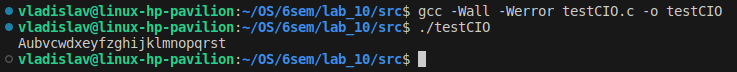
\includegraphics[width=\textwidth]{img/1-1}
	\caption{Результат работы первой программы}
\end{figure}

\captionsetup{singlelinecheck = false, justification=raggedright}
\lstinputlisting[label=lst:author, caption=Первая программа с 2-мя дополнительными потоками, language=c]{../src/testCIO_thread.c}

\begin{figure}[ht]
	\centering
	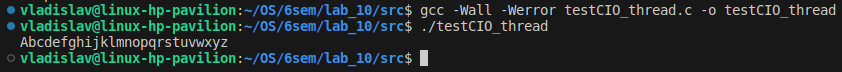
\includegraphics[width=\textwidth]{img/1-2.png}
	\caption{Результат работы первой программы с 2-мя дополнительными потоками}
\end{figure}

\subsection{Анализ результата}

Системный вызов \texttt{open()} открывает файл <<alphabet.txt>> только для чтения
(установлен флаг \texttt{O\_RDONLY}), создает дескриптор открытого файла, соответствующий
индексу в таблице дескрипторов файлов, открытых процессом.  В данном случае
файловому дескриптору присваивается значение 3, так как значения 0, 1, 2 заняты стандартными потоками (\texttt{stdin}, \texttt{stdout},
\texttt{stderr}), а другие файлы процессом не открывались. Поле
\texttt{fd\_array[3]} указывает на \texttt{struct file}, связанную со структурой \texttt{struct inode}, соответствующую файлу <<alphabet.txt>>.

Два вызова \texttt{fdopen()} стандартной библиотеки создают структуры
\texttt{FILE} (\texttt{fs1, fs2}), поле \texttt{\_fileno} которых
инициализируется дескриптором открытого файла.

Вызов функции \texttt{setvbuf()} явно задает буферы для каждой из
структур \texttt{FILE} и их размеры (20~байт), задавая указатели на начало и конец буфера. В данном случае устанавливается буферизация (\texttt{\_IOFBF}).

В цикле поочередно для \texttt{fs1} и \texttt{fs2} вызывается функция
\texttt{fscanf()} стандартной библиотеки. Так как была установлена
буферизация, при первом вызове \texttt{fscanf()} буфер структуры \texttt{fs1}
будет полностью заполнен, то есть в него сразу запишутся первые 20~символов (буквы 'A' -- 't'). При этом, поле \texttt{f\_pos} структуры \texttt{struct file}
установится на следующий символ ('u'), а в переменную \texttt{c} запишется
символ 'A', который и выведется на экран. Вызывая \texttt{fscanf()} для
\texttt{fs2}, в буфер \texttt{fs2} запишутся оставшиеся символы (от 'u' до 'z'), так как
\texttt{fs2} ссылается на тот же дескриптор открытого файла, что и структура \texttt{fs1}, а
поле \texttt{f\_pos} соответствующей структуры \texttt{struct file} было
изменено. В переменную \texttt{c} запишется символ 'u'.

При последующих вызовах \texttt{fscanf()} переменной \texttt{c} будут
присваиваться значения символов из буферов, и попеременно будут выводится
значения из каждого буфера. Когда символы в одном из буферов кончатся,
продолжится вывод символов только из одного буфера.

В случае многопоточной реализации возможны различные варианты вывода, в
зависимости от способа планирования потоков. Возможна
ситуация аналогичная однопоточному варианту, с той поправкой, что порядок вывода
символов разными потоками может отличаться. Возможна также ситуация, при которой главный поток начинает вывод быстрее, так как второму потоку необходимо время на его создание.

\begin{figure}[ht]
	\centering
	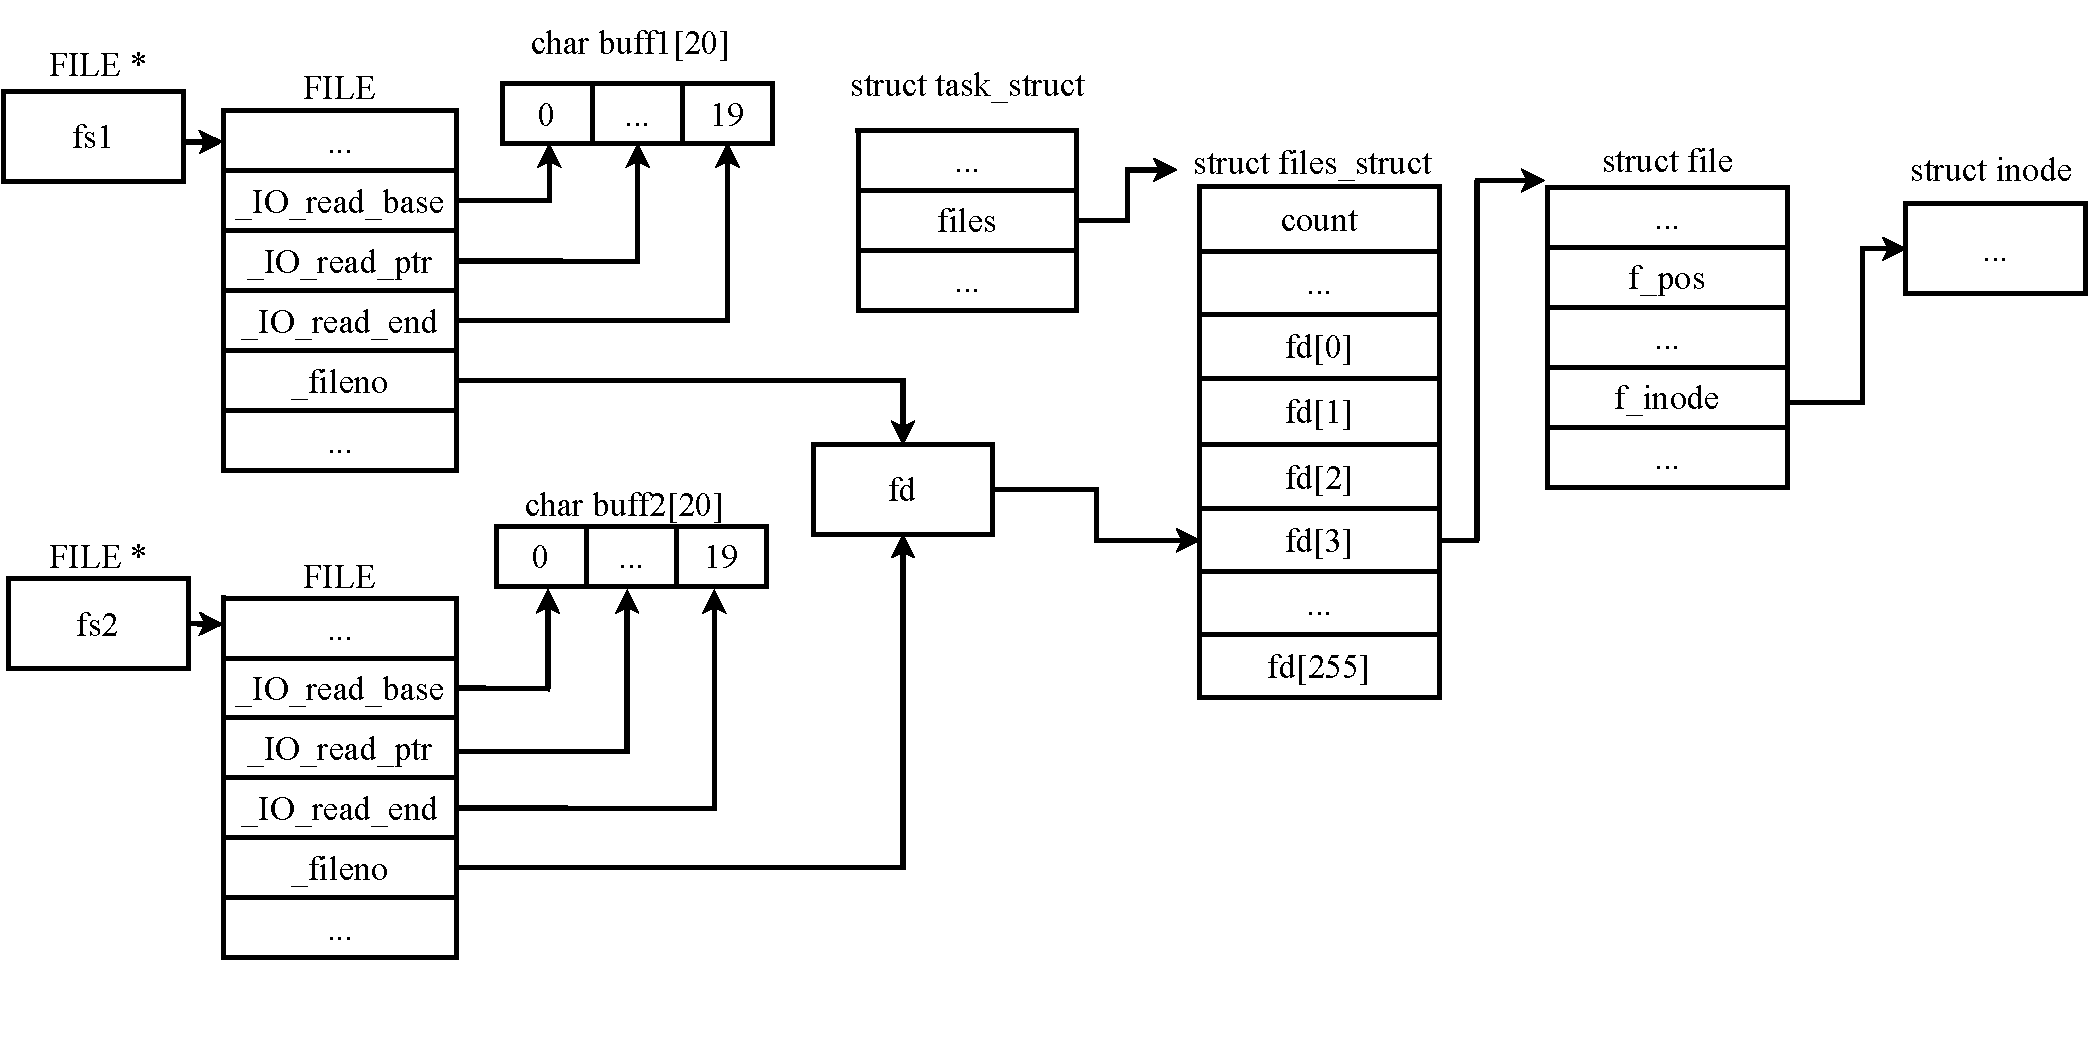
\includegraphics[width=\textwidth]{../data/img/1}
	\caption{Схема связи структур, используемых в первой программе}
\end{figure}\newpage

\section{Вторая программа}

\captionsetup{singlelinecheck = false, justification=raggedright}
\lstinputlisting[label=lst:author, caption=Вторая программа, language=c]{../src/testKernelIO.c}

\begin{figure}[ht]
	\centering
	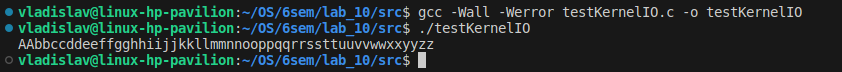
\includegraphics[width=\textwidth]{img/2-1}
	\caption{Результат работы второй программы}
\end{figure}

\captionsetup{singlelinecheck = false, justification=raggedright}
\lstinputlisting[label=lst:author, caption=Вторая программа с дополнительным потоком, language=c]{../src/testKernelIO_thread.c}

\begin{figure}[ht]
	\centering
	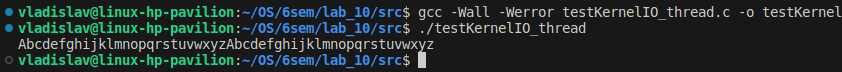
\includegraphics[width=\textwidth]{../data/img/2-2}
	\caption{Результат работы второй программы с дополнительным потоком}
\end{figure}

\subsection{Анализ результата}

Во второй программе посредством двух вызовов \texttt{open()} файл\\ <<alphabet.txt>>
дважды открывается только для чтения (\texttt{O\_RDONLY}), создаются два дескриптора открытого
файла (им присваиваются значения 3 и 4). Вместе с этим, создаются две различные
структуры \texttt{struct file}, ссылающиеся на одну и ту же структуру
\texttt{struct~inode}. Так как структуры \texttt{struct file} разные и их поля
\texttt{f\_pos} изменяются независимо, то для каждого файлового дескриптора
произойдет полное чтение файла и каждый символ будет выведен по два
раза.

При многопоточной реализации алфавит также будет выведен два раза, однако
порядок вывода символов заранее предсказать невозможно.

\begin{figure}[ht]
	\centering
	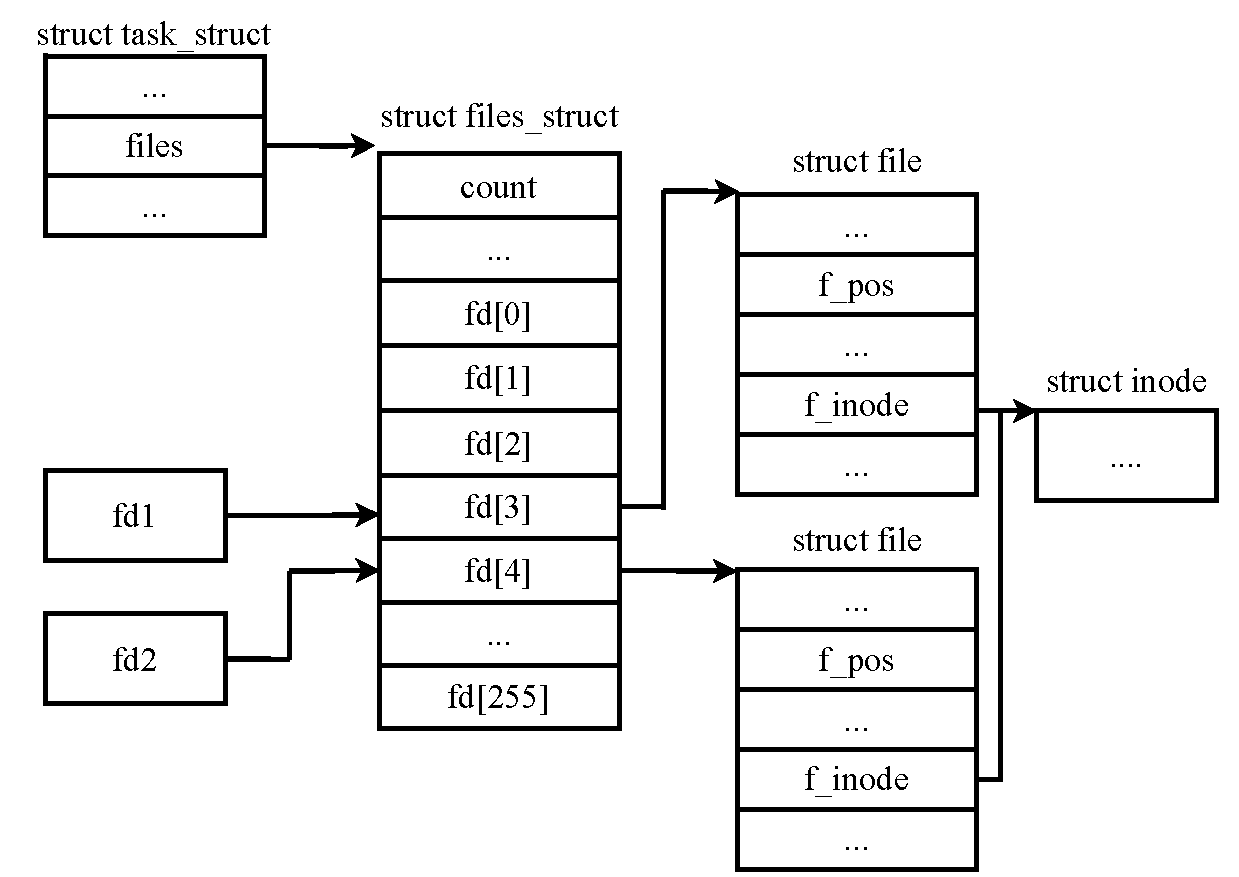
\includegraphics[width=\textwidth]{../data/img/2}
	\caption{Схема связи структур, используемых во второй программе}
\end{figure}\newpage

\section{Третья программа}

\captionsetup{singlelinecheck = false, justification=raggedright}
\lstinputlisting[label=lst:author, caption=Третья программа с fopen, language=c]{../src/test_fopen.c}

\begin{figure}[ht]
	\centering
	\includegraphics[width=\textwidth]{../data/img/3-1}
	\caption{Результат работы третьей программы с fopen}
\end{figure}\newpage

\captionsetup{singlelinecheck = false, justification=raggedright}
\lstinputlisting[label=lst:author, caption=Третья программа с open, language=c]{../src/test_open.c}

\captionsetup{singlelinecheck = false, justification=raggedright}
\lstinputlisting[label=lst:author, caption=езультат работы третьей программы с open, language=bash]{structs/3-2.txt}

\begin{figure}[ht]
	\centering
	\includegraphics[width=\textwidth]{../data/img/3-2}
	\caption{Р}
\end{figure}

\subsection{Анализ результатов}

В третьей программе с использованием \texttt{fopen()} файл дважды открывается для записи (опция <<w>>). Так же, как и во второй программе,
создаются два файловых дескриптора (со значениями 3 и 4), на которые
ссылаются структуры \texttt{FILE} (\texttt{fs1, fs2}) . По умолчанию используется
буферизация, при которой запись в файл из буфера происходит либо когда буфер
заполнен, либо когда вызывается \texttt{fflush}, либо
\texttt{fclose}.

В данном случае, с помощью вывода полей структуры \texttt{struct stat}, можно наблюдать, что запись происходит при вызове \texttt{fclose()}. До
вызовов \texttt{fclose()} в цикле в файл записываются буквы латинского
алфавита с помощью поочередной передачи функции \texttt{fprintf()} дескрипторов.

При вызове \texttt{fclose(fs1)} нечетные буквы алфавита записываются в файл.
При вызове \texttt{fclose(fs2)}, так как поле \texttt{f\_pos}
соответствующей структуры \texttt{struct file} не изменялось, запись в файл
произойдет с начала файла, и записанные ранее символы перезапишутся четными буквами алфавита.
Так как буферы содержали одинаковое количество символов, данные первой
записи утеряны.

В третьей программе с использованием open() результат аналогичный, поскольку установлен флаг \texttt{O\_WRONLY}. Схема связи структур, используемых в третьей программе с open() совпадает с рисунком 6.

Схема связи структур, используемых в третьей программе с fopen(), представлена на рисунке 9.

\begin{figure}[ht]
	\centering
	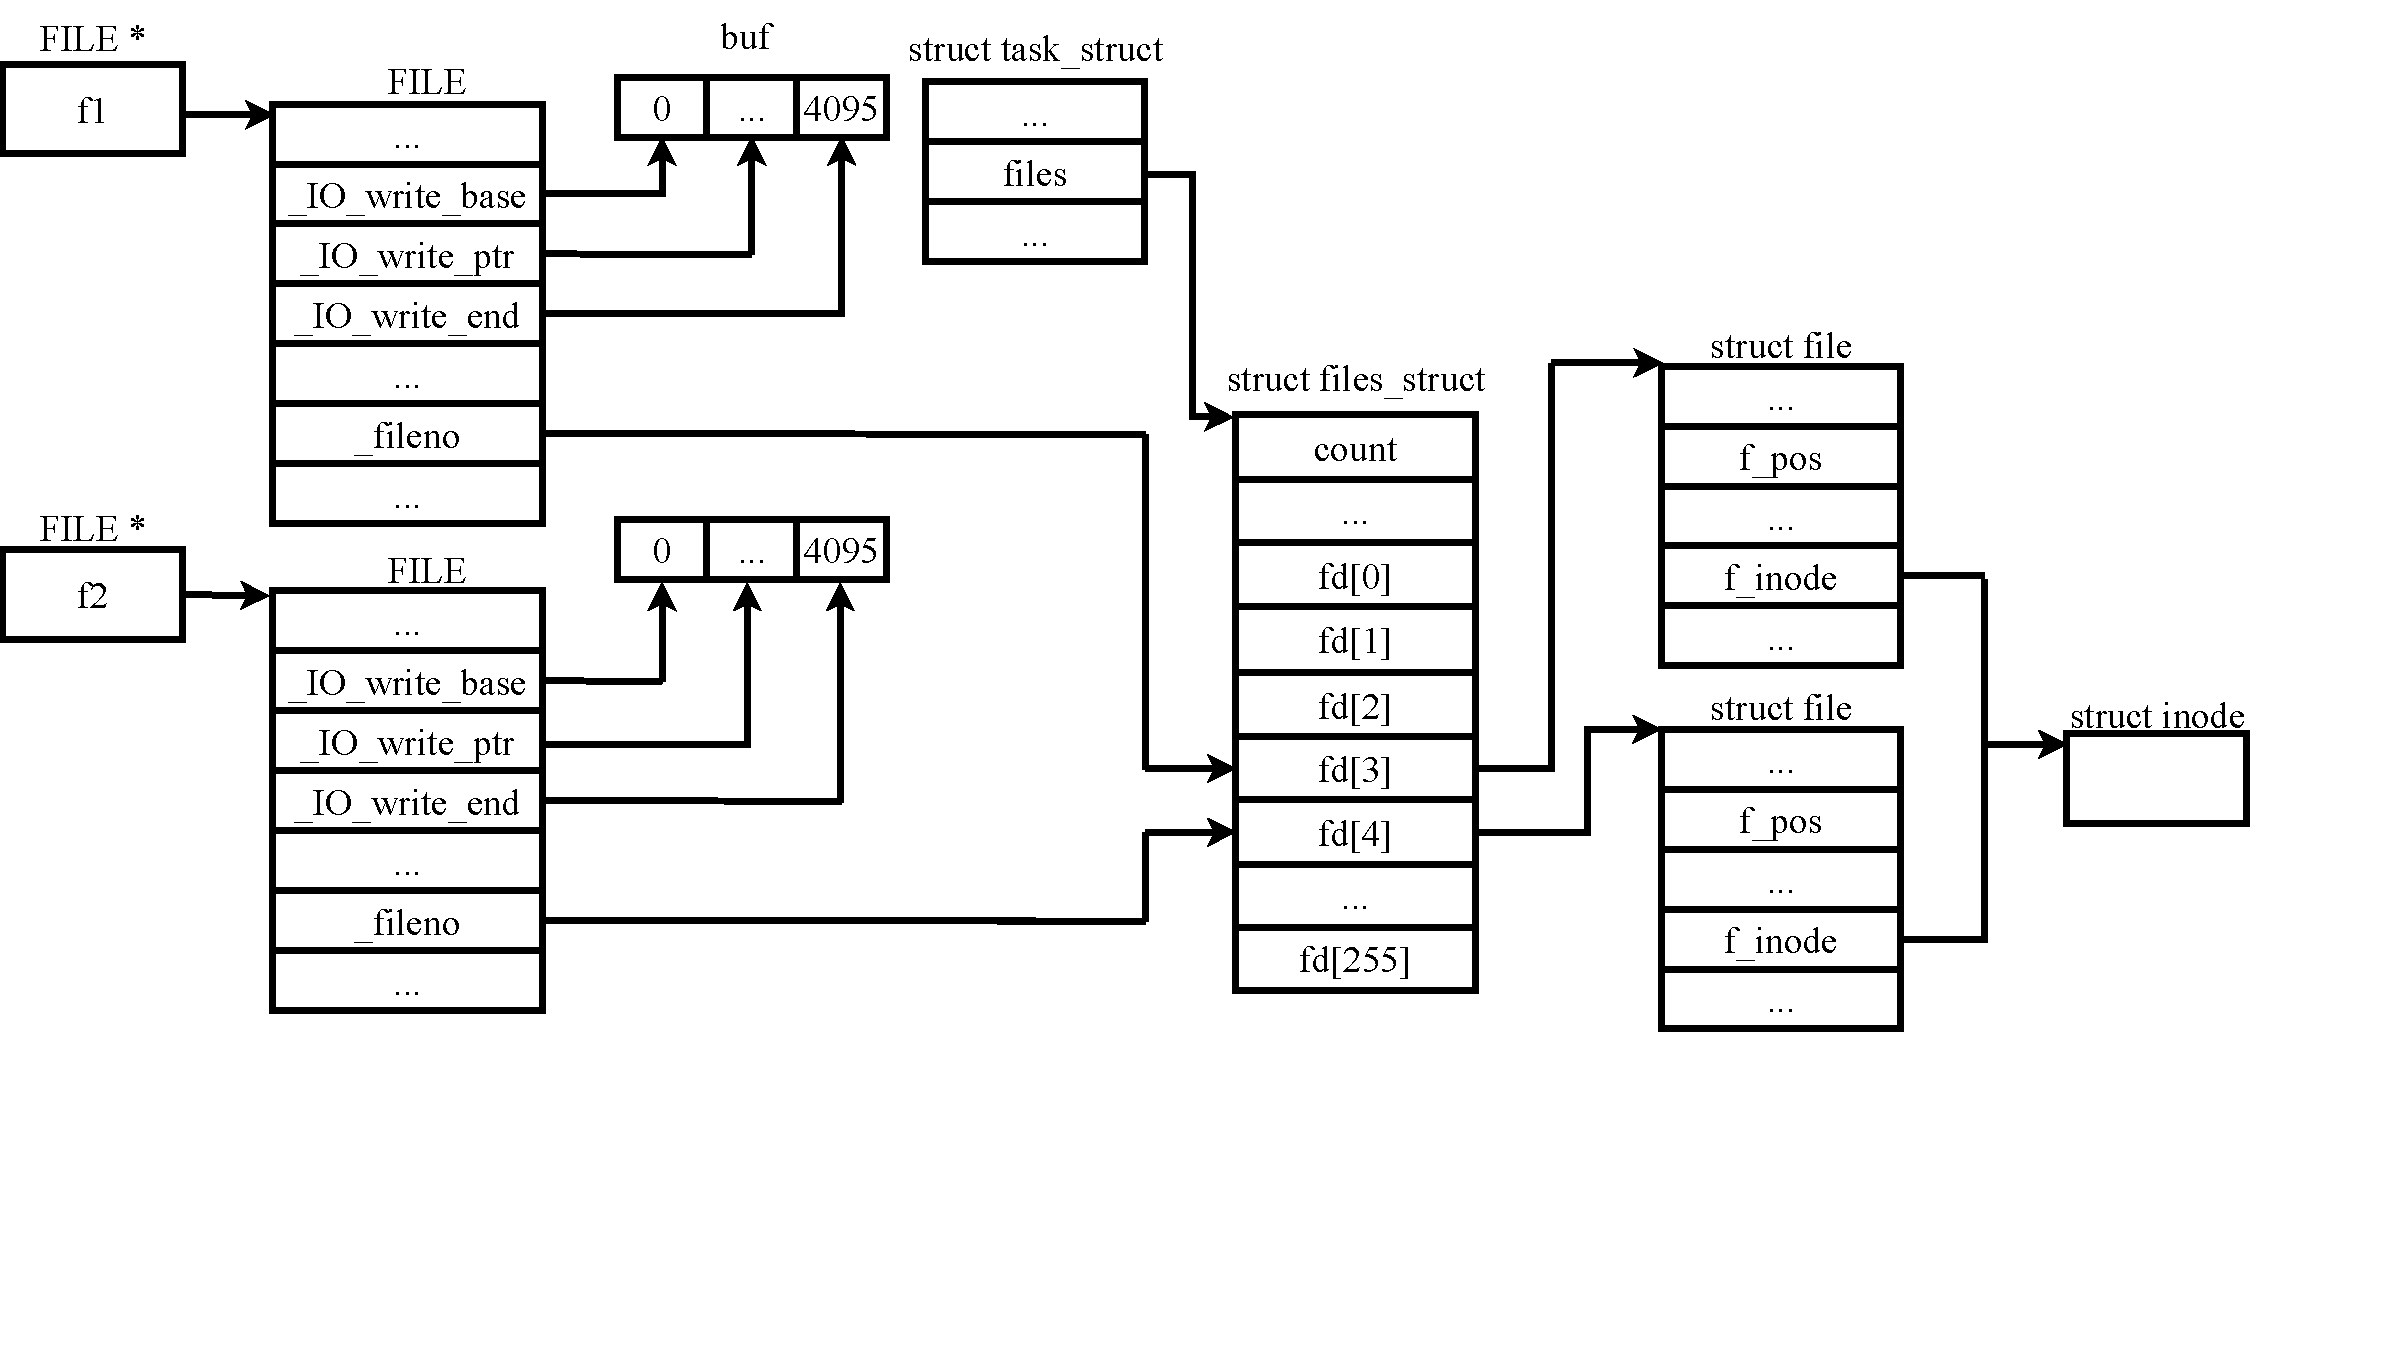
\includegraphics[width=\textwidth]{../data/img/3}
	\caption{Схема связи структур, используемых в третьей программе с fopen}
\end{figure}

Проблема решается добавлением флага \texttt{O\_APPEND} в программу с open() или изменением опции <<w>> на опцию <<a>> в программе с fopen().

